\section{Περιπτώσεις Χρήσης}
\subsection{Εγγραφή χρήστη}

\begin{figure}[H]
  \caption{Εικόνα με Εγγραφή χρήστη.}
  \centering
    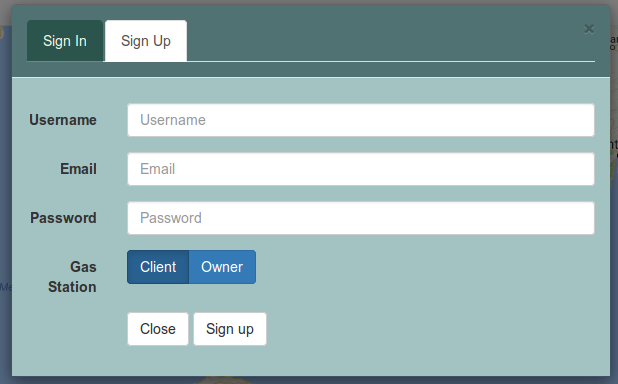
\includegraphics[width=1\textwidth]{img/register.png}
    \label{fig:register}
\end{figure}

\begin{figure}[H]
  \caption{Εικόνα με Εγγραφή χρήστη και λάθος.}
  \centering
    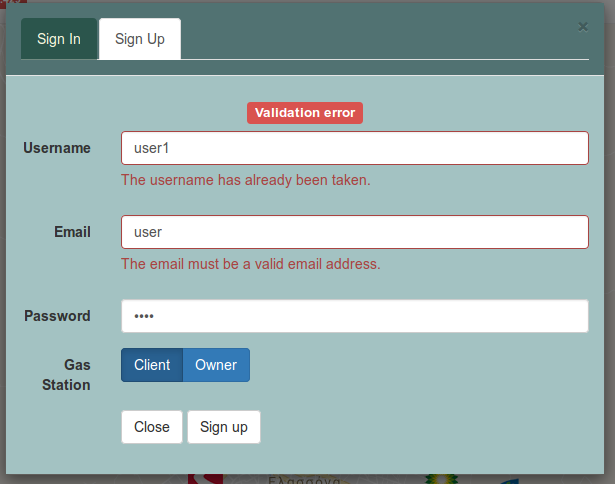
\includegraphics[width=1\textwidth]{img/register-error.png}
    \label{fig:register-error}
\end{figure}

\subsection{LogIn χρήστη}

\begin{figure}[H]
  \caption{Εικόνα με login χρήστη.}
  \centering
    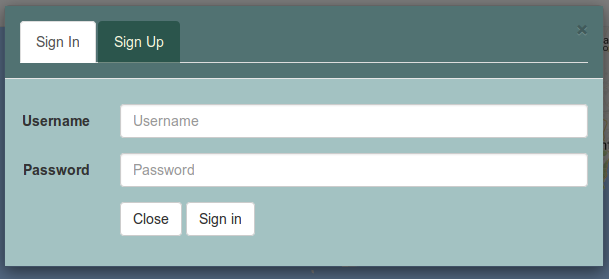
\includegraphics[width=1\textwidth]{img/login.png}
    \label{fig:login}
\end{figure}

\begin{figure}[H]
  \caption{Εικόνα με login χρήστη και λάθος.}
  \centering
    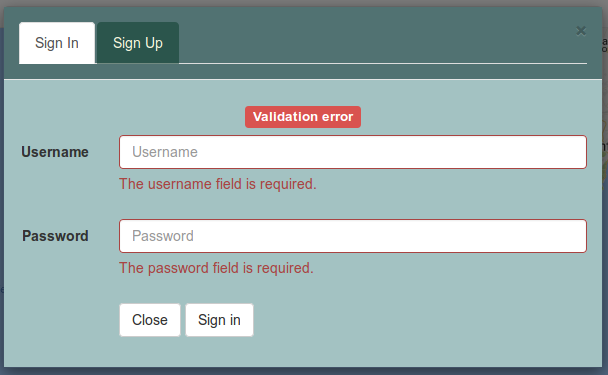
\includegraphics[width=1\textwidth]{img/login-error.png}
    \label{fig:login-error}
\end{figure}

\begin{figure}[H]
  \caption{Εικόνα με login χρήστη success.}
  \centering
    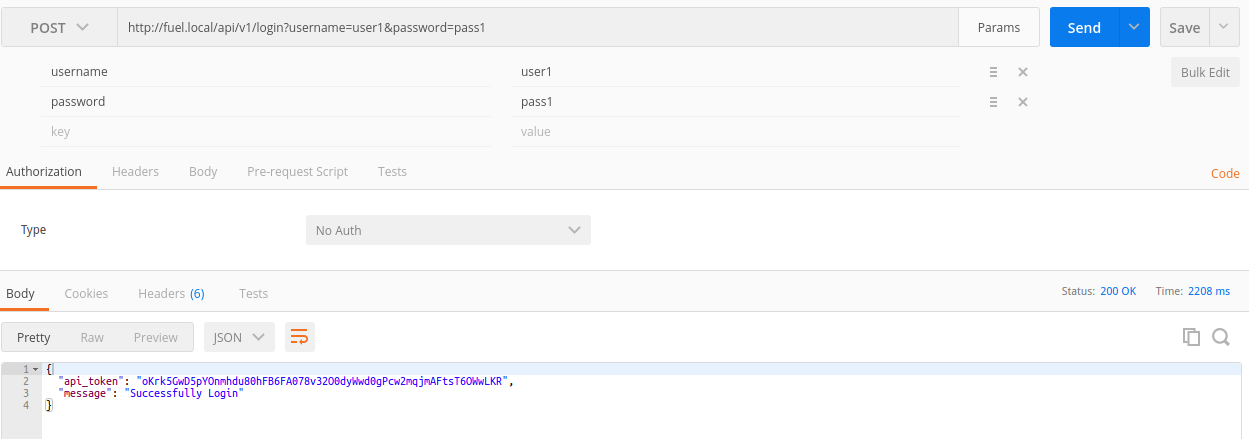
\includegraphics[width=1\textwidth]{img/login-post.png}
    \label{fig:login-post}
\end{figure}

\subsection{Πλήθος πρατηρίων}

\begin{figure}[H]
  \caption{Εικόνα με το Πλήθος πρατηρίων.}
  \centering
    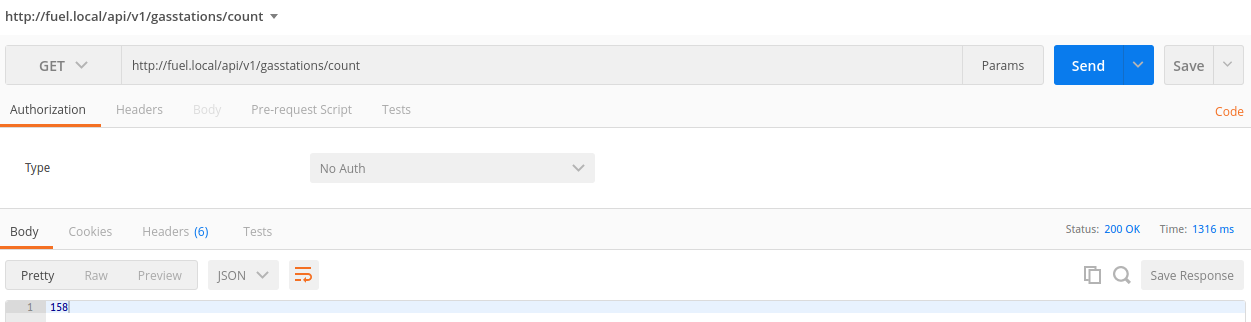
\includegraphics[width=1\textwidth]{img/count.png}
    \label{fig:count}
\end{figure}

\subsection{Λήψη μέγιστης, ελάχιστης και μέσης τιμής}

\begin{figure}[H]
  \caption{Εικόνα μέγιστης, ελάχιστης και μέσης τιμής από την εφαρμογή.}
  \centering
    
\includegraphics[width=1\textwidth]{img/max-min.png}
    \label{fig:max-min}
\end{figure}

\begin{figure}[H]
  \caption{Εικόνα μέγιστης, ελάχιστης και μέσης τιμής από το request.}
  \centering
    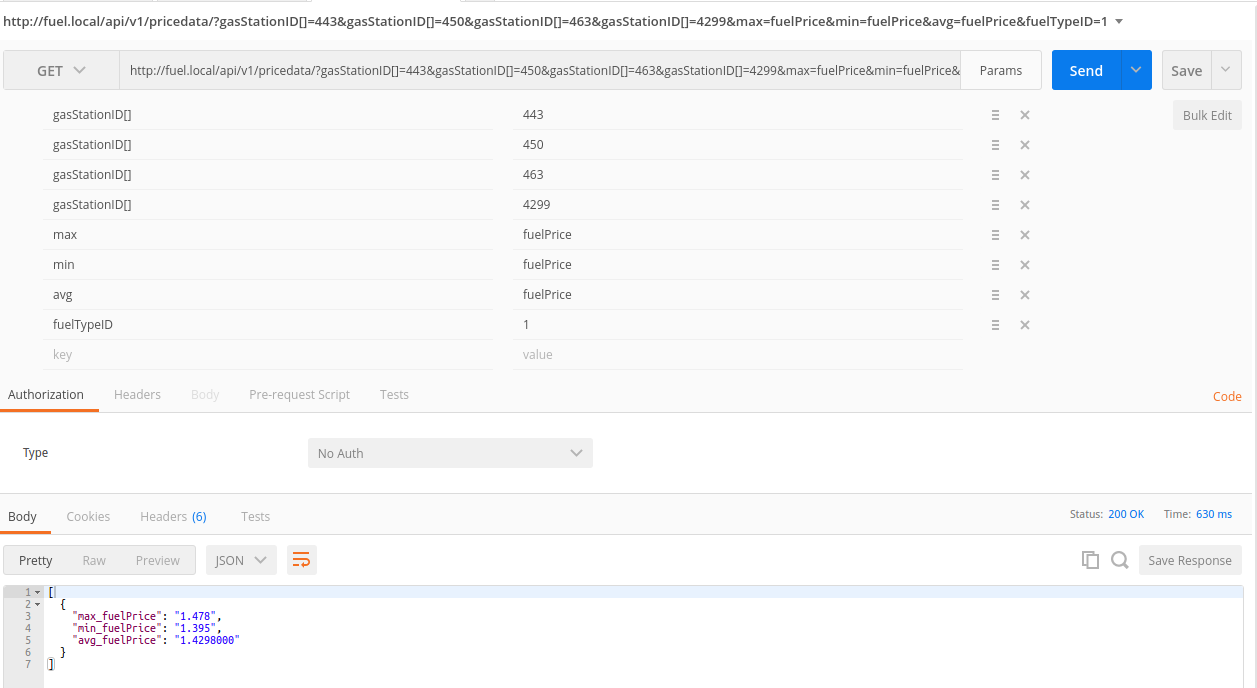
\includegraphics[width=1\textwidth]{img/max-min-postman.png}
    \label{fig:max-min-postman}
\end{figure}

\subsection{Λήψη τιμοκαταλόγου πρατηρίου}

\begin{figure}[H]
  \caption{Εικόνα πριν από τη λήψη τιμοκαταλόγου πρατηρίου.}
  \centering
    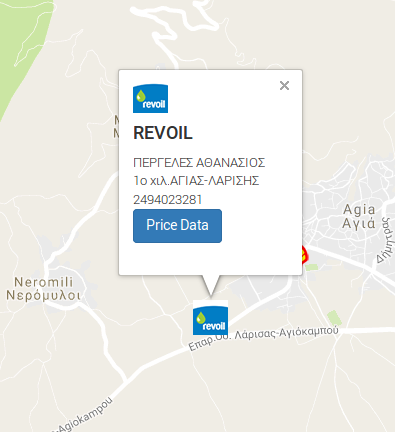
\includegraphics[width=1\textwidth]{img/pricedata1.png}
    \label{fig:pricedata1}
\end{figure}

\begin{figure}[H]
  \caption{Εικόνα μετά από τη λήψη τιμοκαταλόγου πρατηρίου.}
  \centering
    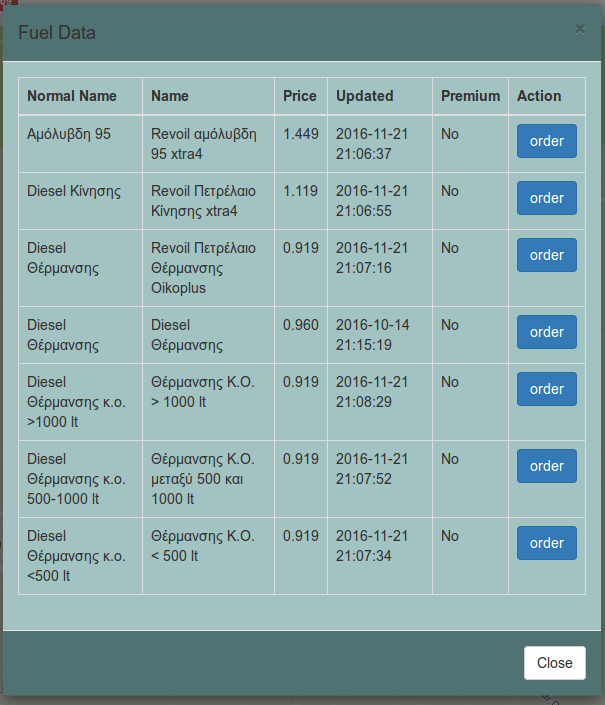
\includegraphics[width=1\textwidth]{img/pricedata2.png}
    \label{fig:pricedata2}
\end{figure}

\begin{figure}[H]
  \caption{Εικόνα με τη λήψη τιμοκαταλόγου πρατηρίου  από το request.}
  \centering
    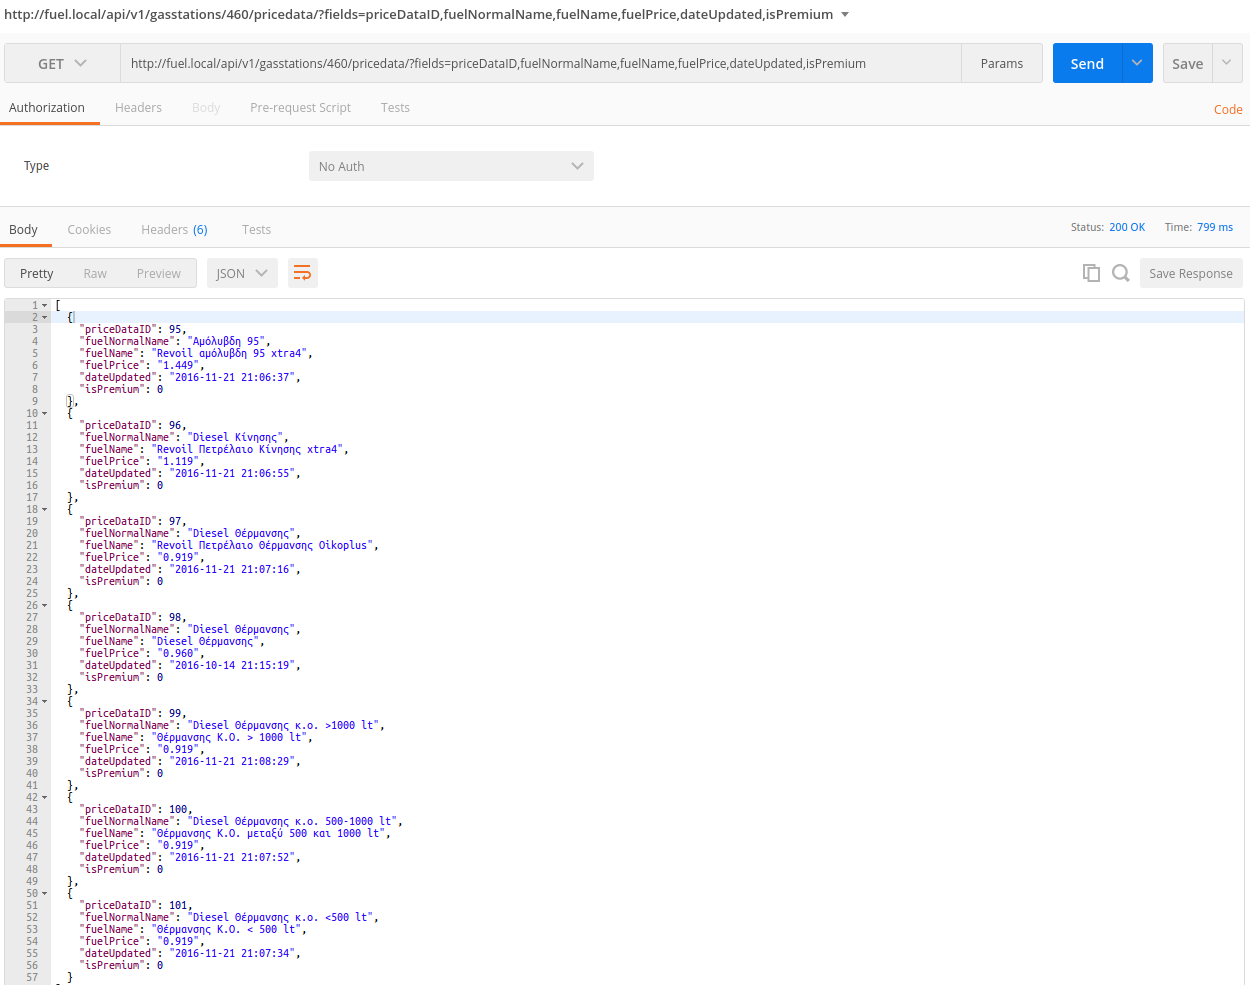
\includegraphics[width=1\textwidth]{img/pricedata3.png}
    \label{fig:pricedata3}
\end{figure}

\subsection{Λήψη δεδομένων πρατηρίων}

\begin{figure}[H]
  \caption{Εικόνα με τη λήψη δεδομένων πρατηρίων από το request.}
  \centering
    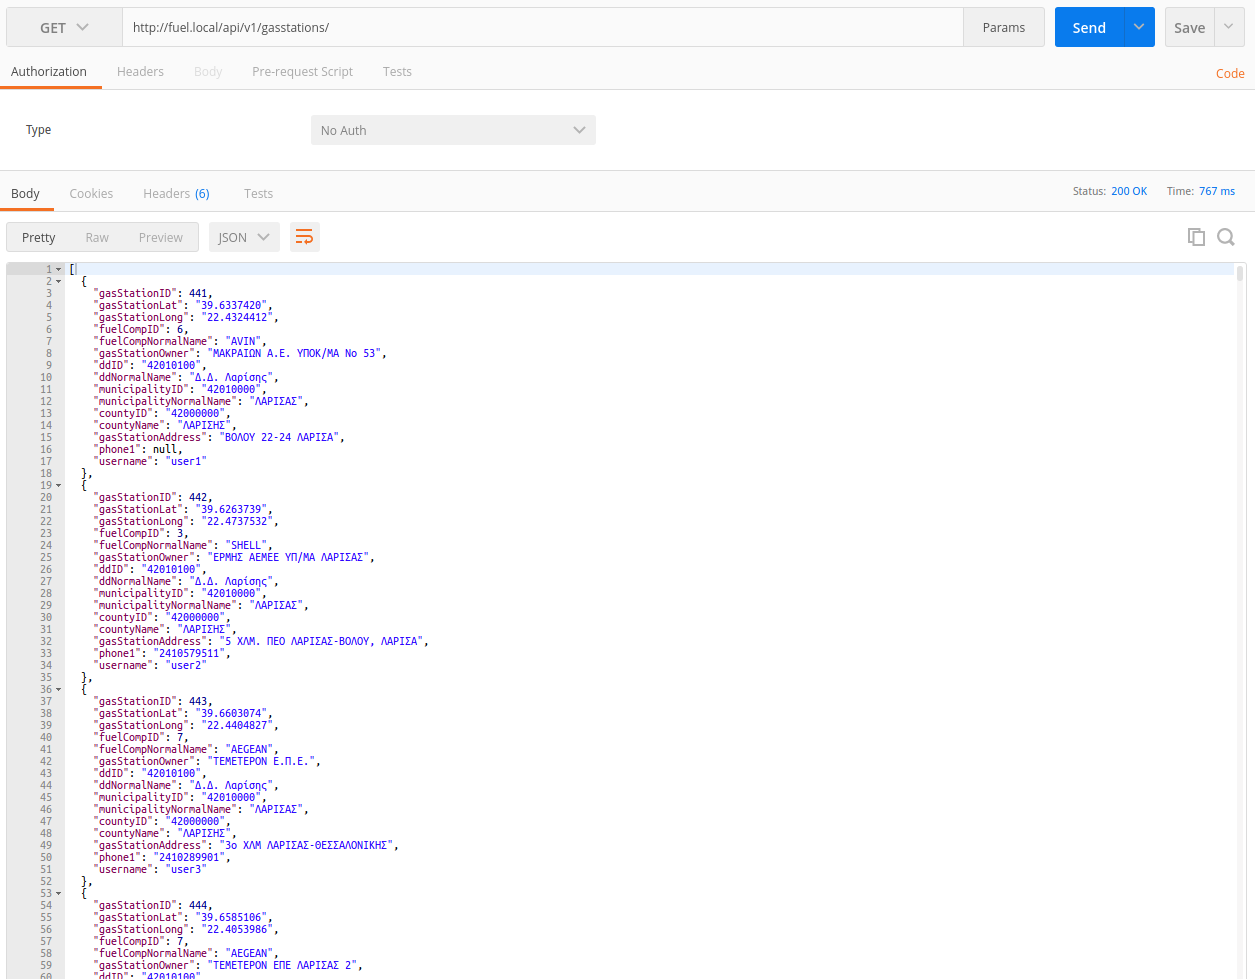
\includegraphics[width=1\textwidth]{img/gasstations.png}
    \label{fig:gasstations}
\end{figure}

\subsection{Έλεγχος παραγγελιών από πρατηριούχο}

\begin{figure}[H]
  \caption{Εικόνα με πριν τον ελεγχο παραγγελιών από πρατηριούχο.}
  \centering
    
\includegraphics[width=1\textwidth]{img/pre-orders.png}
    \label{fig:pre-orders}
\end{figure}

\begin{figure}[H]
  \caption{Εικόνα κατά τον ελεγχο παραγγελιών από πρατηριούχο.}
  \centering
    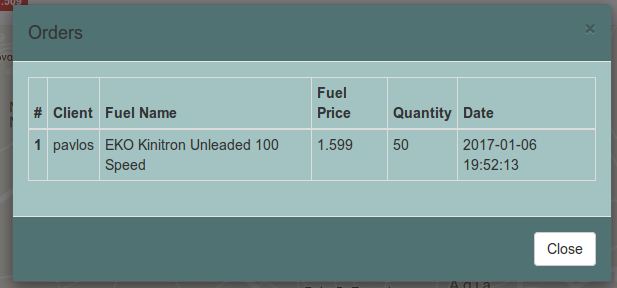
\includegraphics[width=1\textwidth]{img/orders.png}
    \label{fig:orders}
\end{figure}

\subsection{Ενημέρωση τιμών στο σύστημα από πρατηριούχους}

\begin{figure}[H]
  \caption{Εικόνα πριν την ενημέρωση τιμών.}
  \centering
    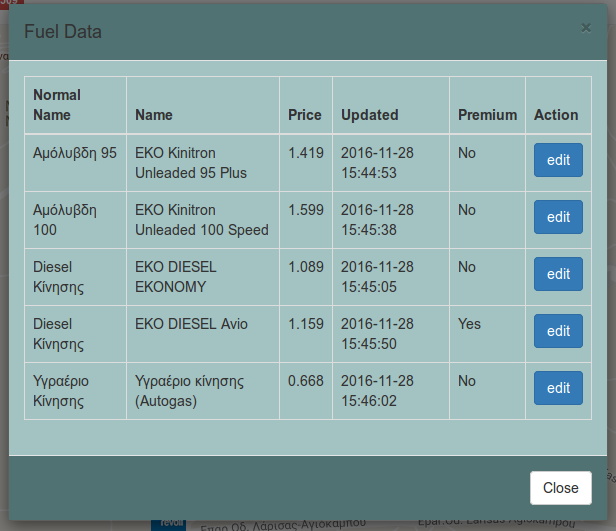
\includegraphics[width=1\textwidth]{img/pre-edit.png}
    \label{fig:pre-edit}
\end{figure}

\begin{figure}[H]
  \caption{Εικόνα κατά την ενημέρωση τιμών.}
  \centering
    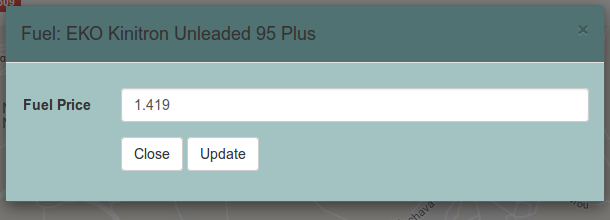
\includegraphics[width=1\textwidth]{img/pre-edit2.png}
    \label{fig:pre-edit2}
\end{figure}

\begin{figure}[H]
  \caption{Εικόνα μηνύματος μετά από την ενημέρωση τιμών.}
  \centering
    
\includegraphics[width=1\textwidth]{img/msg-edit.png}
    \label{fig:msg-edit}
\end{figure}

\begin{figure}[H]
  \caption{Εικόνα μετά από την ενημέρωση τιμών.}
  \centering
    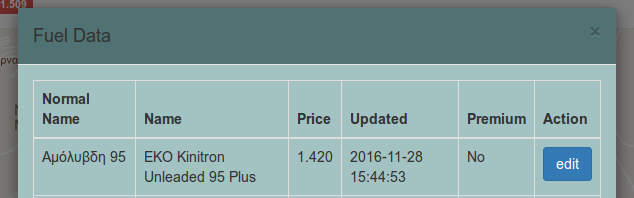
\includegraphics[width=1\textwidth]{img/after-edit.png}
    \label{fig:after-edit}
\end{figure}

\subsection{Αποστολή δεδομένων παραγγελίας από πλευράς χρήστη}

Εικόνα πριν την Αποστολή παραγγελίας. \ref{fig:pricedata1}

\begin{figure}[H]
  \caption{Εικόνα Login error κατά την Αποστολή παραγγελίας.}
  \centering
    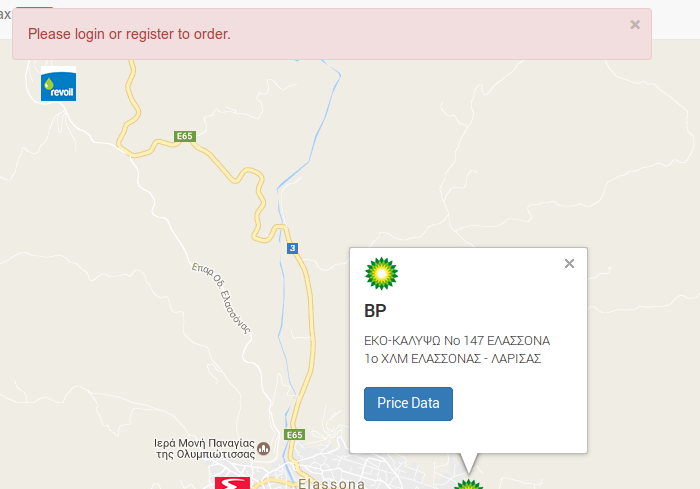
\includegraphics[width=1\textwidth]{img/make-order-error.png}
    \label{fig:make-order-error}
\end{figure}

\begin{figure}[H]
  \caption{Εικόνα quantity error κατά την Αποστολή παραγγελίας.}
  \centering
    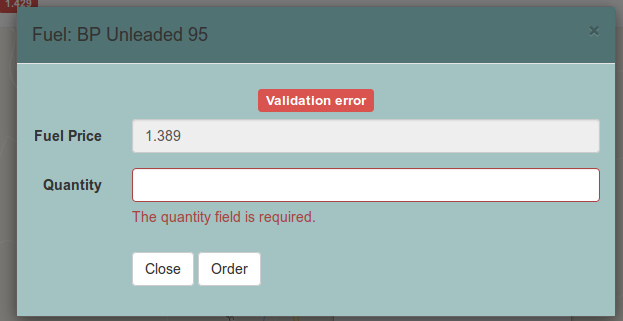
\includegraphics[width=1\textwidth]{img/make-order-error2.png}
    \label{fig:make-order-error2}
\end{figure}

\subsection{Επιλογή default fuel type για την απεικόνιση των max, min, avg τιμών}

\begin{figure}[H]
  \caption{Εικόνα επιλογής default fuel type.}
  \centering
    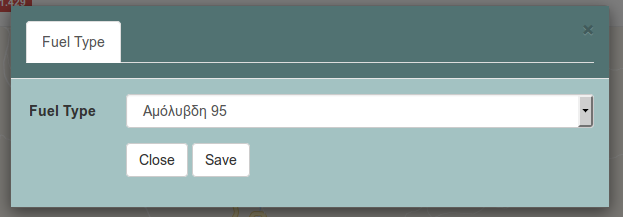
\includegraphics[width=1\textwidth]{img/fuel-type.png}
    \label{fig:fuel-type}
\end{figure}

\subsection{Μεταβίβαση σε επιλεγμένη περιοχή}

\begin{figure}[H]
  \caption{Εικόνα λάθους μεταβίβαση σε επιλεγμένη περιοχή.}
  \centering
    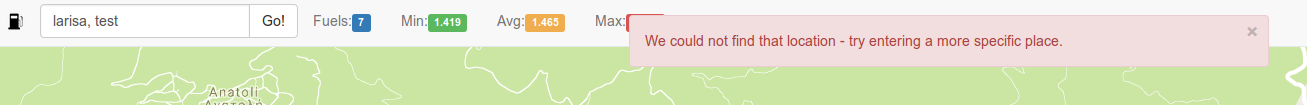
\includegraphics[width=1\textwidth]{img/area-error.png}
    \label{fig:arrea-error}
\end{figure}

\begin{figure}[H]
  \caption{Εικόνα πριν την μεταβίβαση σε επιλεγμένη περιοχή.}
  \centering
    
\includegraphics[width=1\textwidth]{img/pre-area.png}
    \label{fig:pre-area}
\end{figure}

\begin{figure}[H]
  \caption{Εικόνα κατά την μεταβίβαση σε επιλεγμένη περιοχή.}
  \centering
    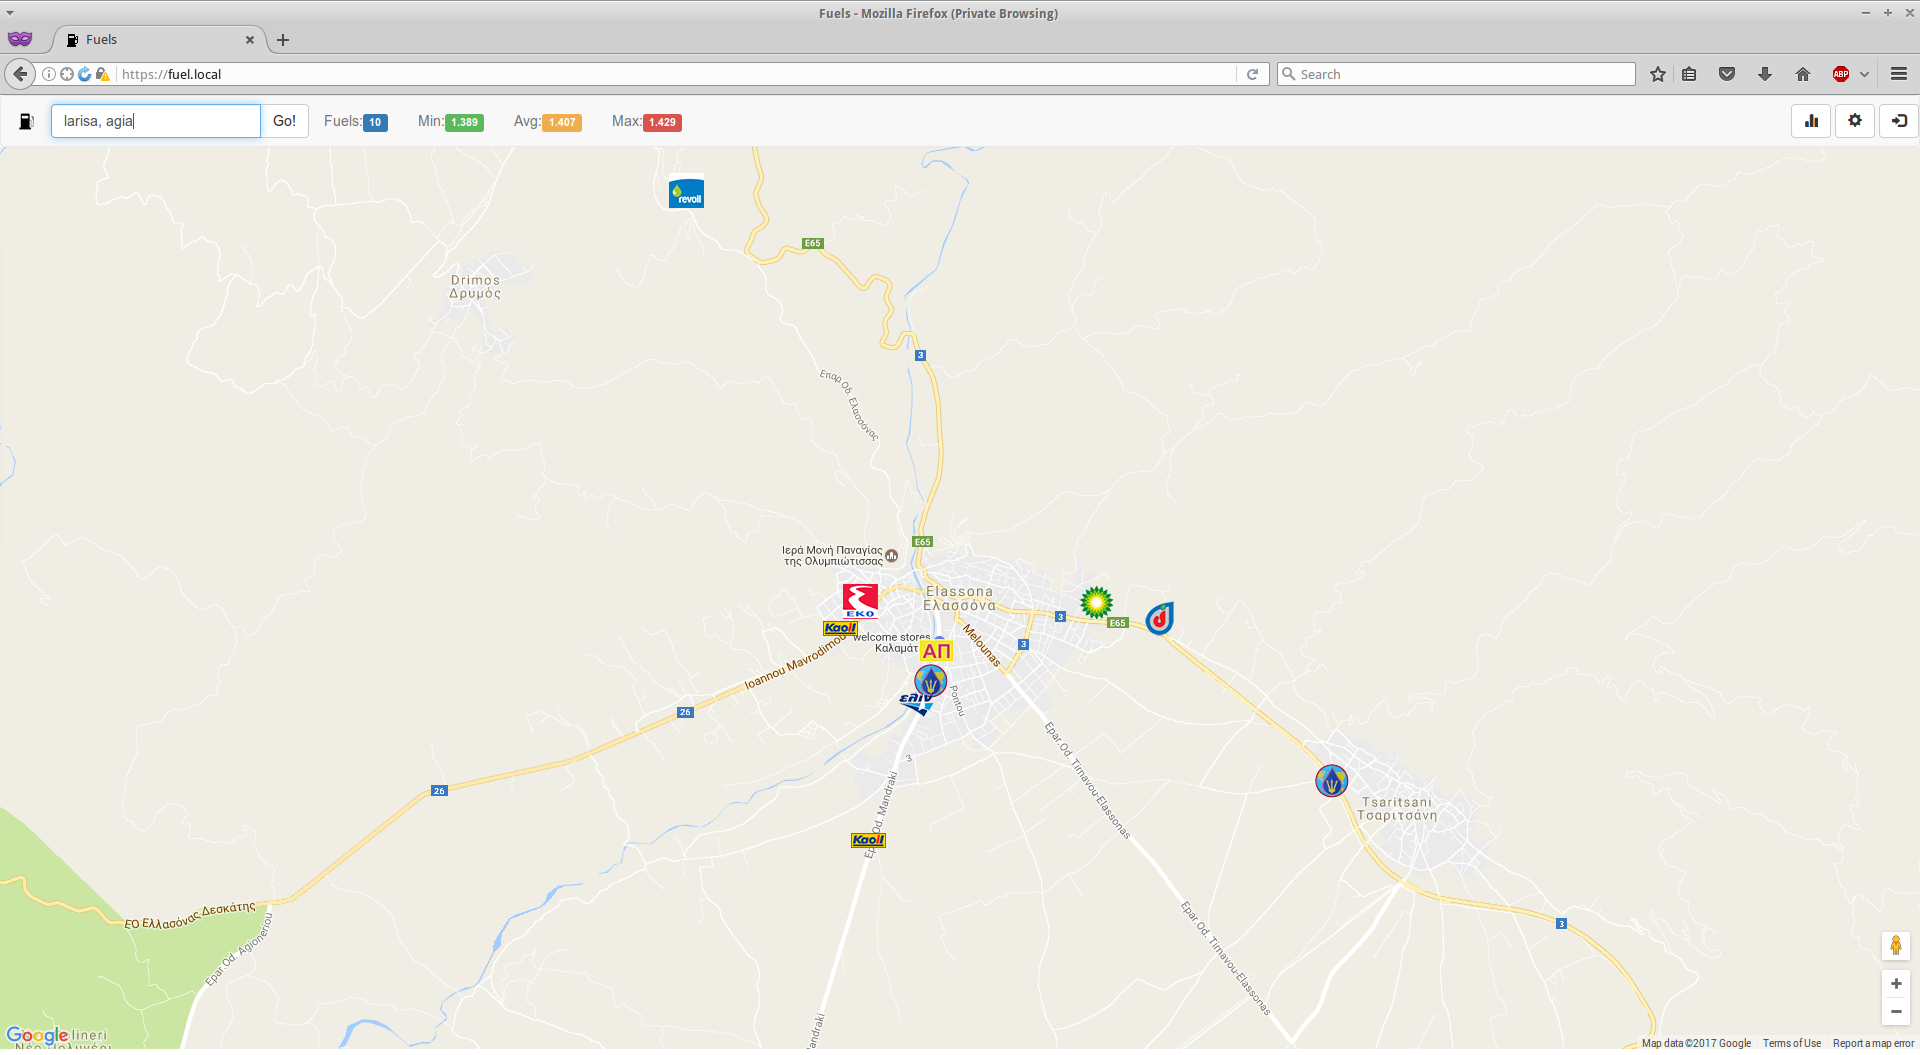
\includegraphics[width=1\textwidth]{img/area.png}
    \label{fig:area}
\end{figure}

\begin{figure}[H]
  \caption{Εικόνα μετά την μεταβίβαση σε επιλεγμένη περιοχή.}
  \centering
    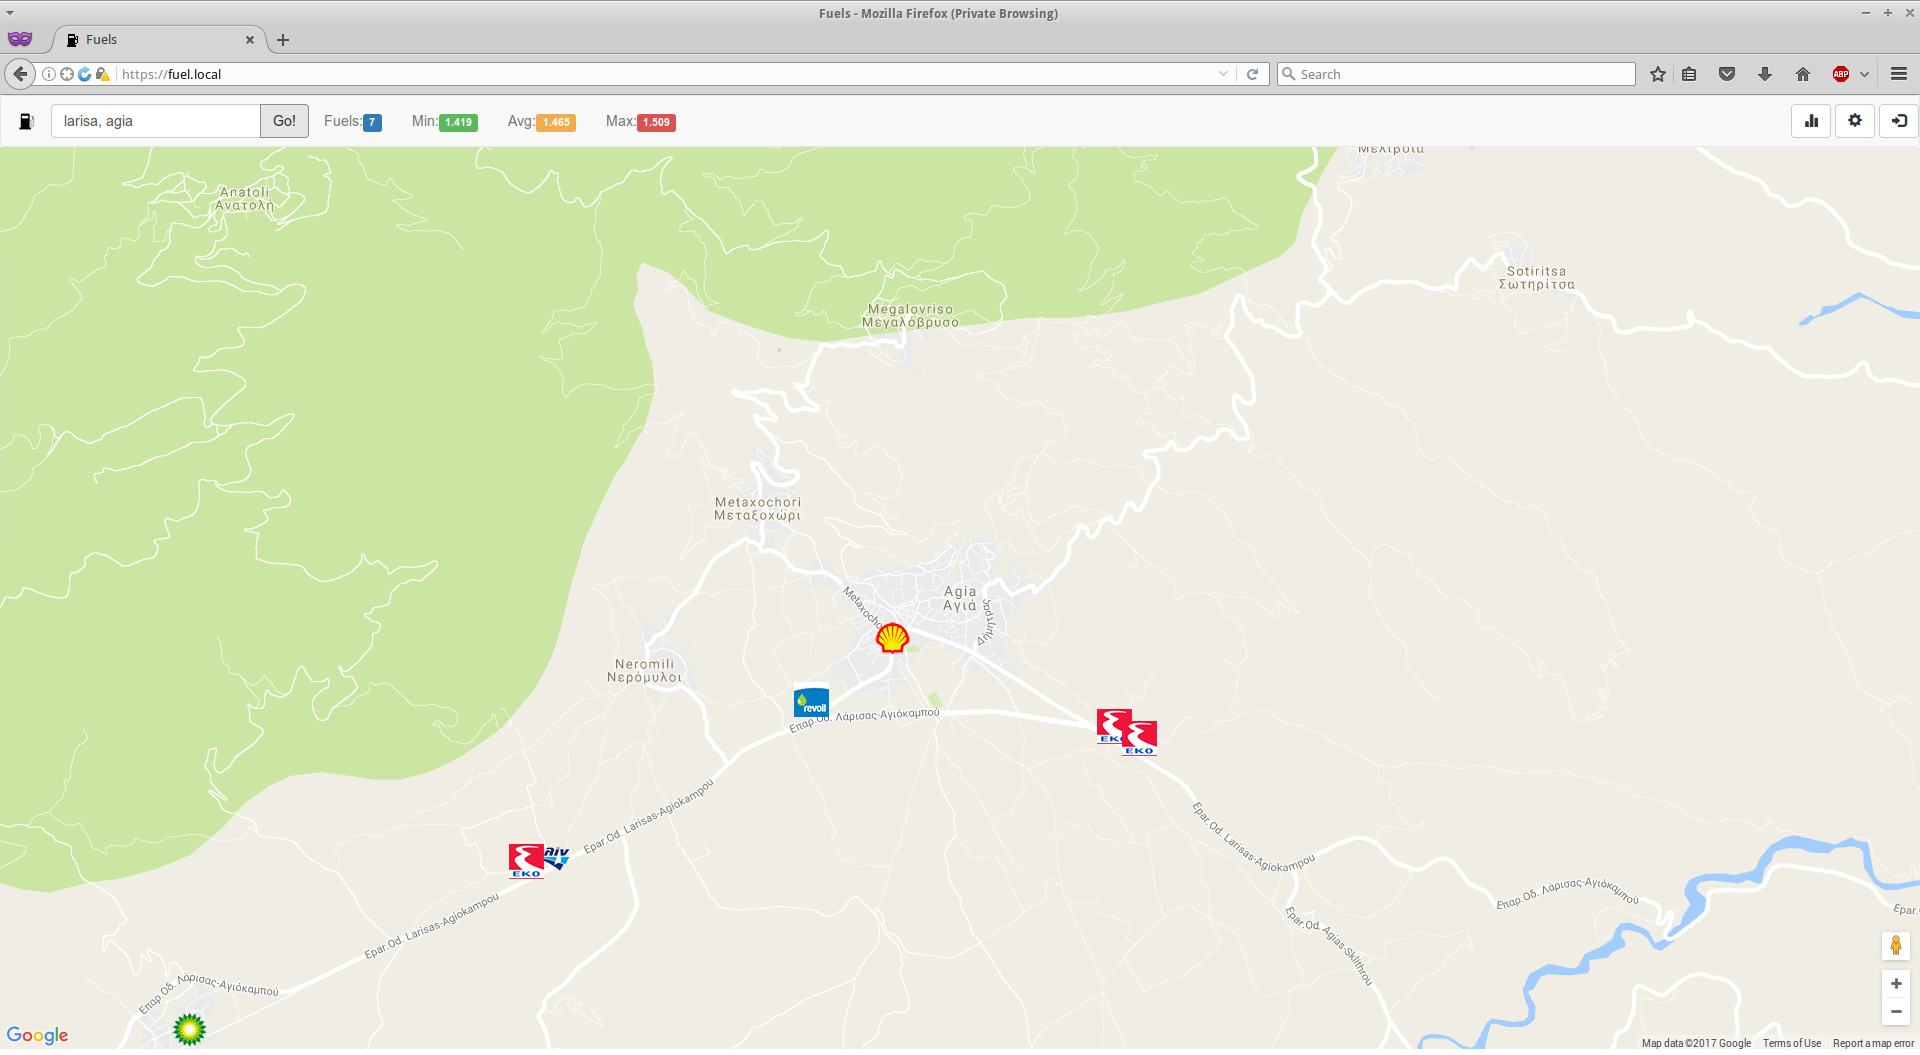
\includegraphics[width=1\textwidth]{img/area-after.png}
    \label{fig:area-after}
\end{figure}

\subsection{Επιλογή Geolocation}

\begin{figure}[H]
  \caption{Εικόνα κατά την Επιλογή Geolocation.}
  \centering
    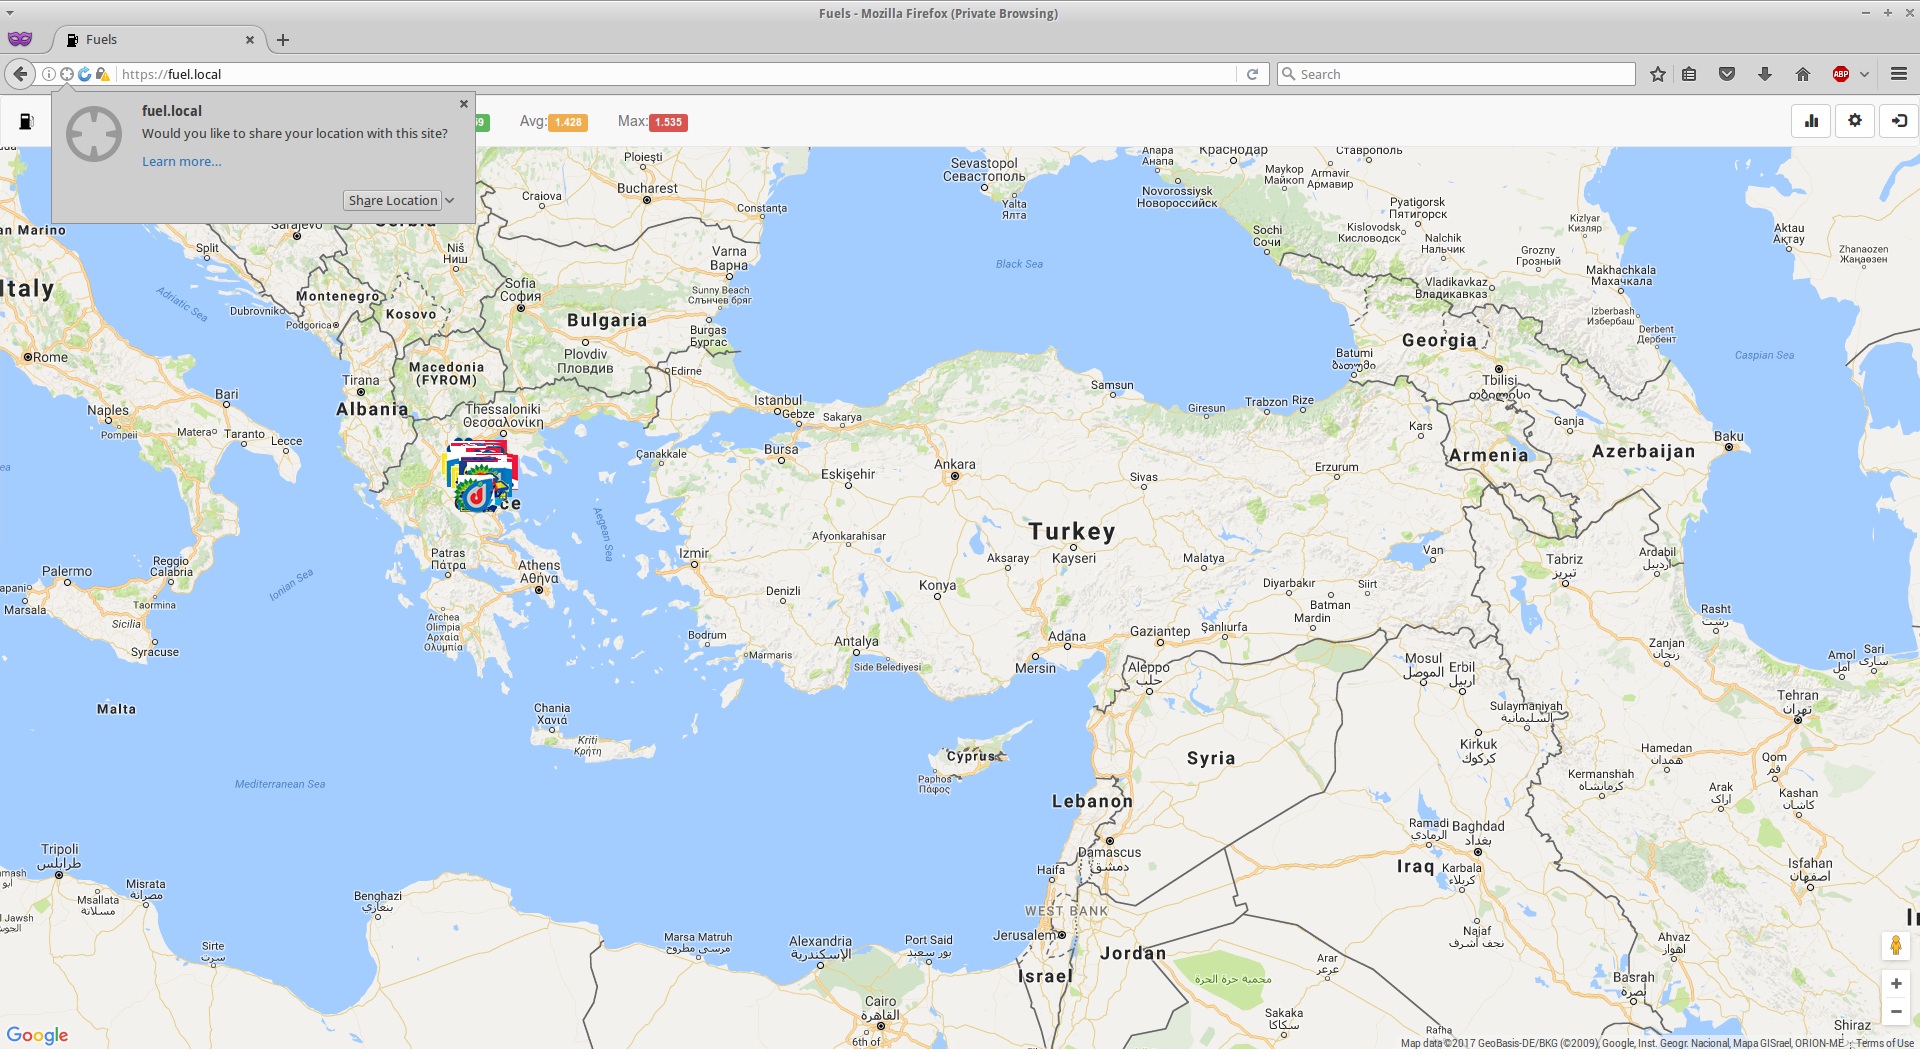
\includegraphics[width=1\textwidth]{img/geolocation.png}
    \label{fig:geolocation}
\end{figure}

Τα μηνύματα των φορμών καθώς και τα notifications προέρχονται κυρίως από το REST API.